\documentclass[border=10pt]{standalone}
\usepackage{xcolor}
\usepackage{tikz}
\usetikzlibrary{arrows.meta,positioning,fit,backgrounds}

\definecolor{BG}{HTML}{FAFAFA}
\definecolor{INK}{HTML}{1A1A2E}
\definecolor{SUB}{HTML}{555566}
\definecolor{COLD}{HTML}{4361EE}
\definecolor{WARM}{HTML}{2EC4B6}
\definecolor{NEW}{HTML}{F4A261}

\begin{document}
\pagecolor{BG}
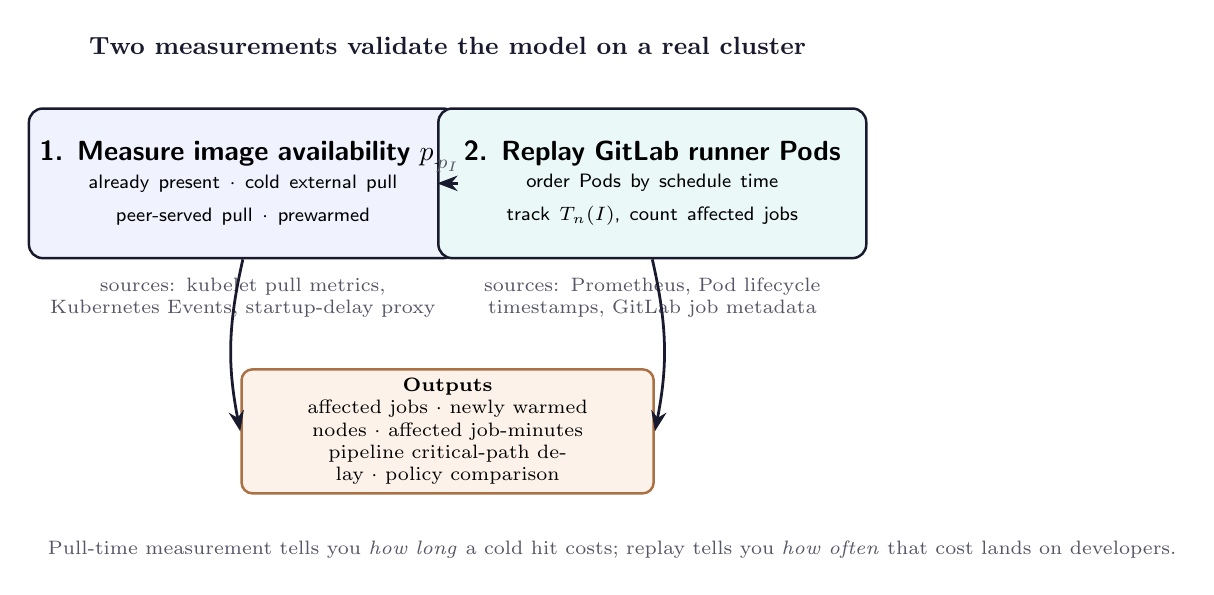
\begin{tikzpicture}[
  font=\sffamily,
  box/.style={rounded corners=5pt, draw=INK, line width=0.9pt, align=center, minimum height=1.9cm, text width=5.2cm},
  m1/.style={box, fill=COLD!8},
  m2/.style={box, fill=WARM!10},
  outbox/.style={rounded corners=4pt, draw=NEW!70!black, line width=0.9pt, fill=NEW!14, align=center, text width=5.0cm, font=\scriptsize},
  arr/.style={-{Stealth[length=2.6mm]}, draw=INK, line width=1.0pt},
  head/.style={font=\small\bfseries, text=INK},
  sub/.style={font=\scriptsize, text=SUB},
]

\node[head] at (5.4, 4.35) {Two measurements validate the model on a real cluster};

% Measurement 1
\node[m1] (m1) at (2.8, 2.6) {%
  {\bfseries 1. Measure image availability \(p_I\)}\\[2pt]
  \scriptsize already present \(\cdot\) cold external pull\\
  \scriptsize peer-served pull \(\cdot\) prewarmed};
\node[sub, text width=5.2cm, align=center] at (2.8, 1.15)
  {sources: kubelet pull metrics,\\Kubernetes Events, startup-delay proxy};

% Measurement 2
\node[m2] (m2) at (8.0, 2.6) {%
  {\bfseries 2. Replay GitLab runner Pods}\\[2pt]
  \scriptsize order Pods by schedule time\\
  \scriptsize track \(T_n(I)\), count affected jobs};
\node[sub, text width=5.2cm, align=center] at (8.0, 1.15)
  {sources: Prometheus, Pod lifecycle\\timestamps, GitLab job metadata};

% p_I feeds replay
\draw[arr] (m1.east) -- node[above, sub, font=\scriptsize\bfseries] {\(p_I\)} (m2.west);

% output
\node[outbox] (out) at (5.4, -0.55) {%
  {\bfseries Outputs}\\
  affected jobs \(\cdot\) newly warmed nodes \(\cdot\) affected job-minutes\\
  pipeline critical-path delay \(\cdot\) policy comparison};
\draw[arr] (m1.south) to[bend right=12] (out.west);
\draw[arr] (m2.south) to[bend left=12] (out.east);

\node[sub, anchor=west] at (0.2, -2.05)
  {Pull-time measurement tells you \emph{how long} a cold hit costs; replay tells you \emph{how often} that cost lands on developers.};

\end{tikzpicture}
\end{document}
